
\chapter{目前存在的震级预估方法简介}

\section{预估震级的可能性}

\indent 能够由初始破裂信息估计出整个地震的规模是预估震级可行的基本前提。目前学术界对于这个问题仍没有一致性的认识。持否定态度的学者认为破裂过程在时序上是不可预测,即使用已得到的地震台信息只能评估目前的地震释放的能量但不能预估整个断层破裂结束所释放的能量大小(Mori, 1996; Kilb et al, 1999),。但仍有已有多种观点支持根据少量初始信息进行地震震级预估是可行的。首先,在断层初始破裂过程中存在成核震相,而它直接决定了最终破裂的形态 (Ellsworth and Beroza, 1995; 马胜利等, 2002; Dodge et al, 1996);其次,地震产生的P波和S波分别携带不同信息,前者携带着反映断层如何滑动的信息,而后者则携带着地震能量的信息,因此可以分别加以利用,在破坏性较强的S波到来之前,通过P波的特征估计出断层破裂信息 (Beroza et al, 1995)。
在这此问题的不断争论中,已有许多研究成果表明在一定的精度要求下是可以做到使用初始破裂信息估计整个地震的规模的 (Allen et al., 2003, 2007; Kanamori et al., 1997, 2005, 2008)。根据不同算法的出发点,大致可以划分为两类,分别是特征频率类方法和特征振幅类方法。\\

\section{特征频率类方法}
\indent 对于估计地震规模的问题,最重要的是确定地震的破裂是否已经停止,或者是仍持续扩展,特征频率类方法就是通过最初的地表震动周期长短来判定地震破裂的持续情况 (Kanamori, 2005; Allen, 2005)。尽管事实上地震破裂的过程往往很复杂,甚至一个大规模地震初始是由一个短周期的初动持续作用引起的,但这并不影响我们从平均意义上研究地震的特征周期(或特征频率)与最终地震规模的关系。\\

\indent Nakamura (1988) 首先提出了利用实时速度记录计算地震动卓越周期的算法,随后经一些研究者拓展形成了对P波拐角频率的特征进行估计的$\tau_{p}^{\max }$方法 (Allen et al, 2003; Olson et al., 2005; Kanamori et al., 1995, 2005)。根据这种方法,\\
\begin{equation}
\tau_{\mathrm{i}}^{\mathrm{p}}=2 \pi \sqrt{\frac{\mathrm{X}_{\mathrm{i}}}{\mathrm{D}_{\mathrm{i}}}}
\end{equation}
式中,$\mathrm{X}_{\mathrm{i}}=\alpha \mathrm{X}_{\mathrm{i}-1}+\mathrm{x}_{\mathrm{i}}^{2}, \mathrm{D}_{\mathrm{i}}=\alpha \mathrm{D}_{\mathrm{i}-1}+\left(\frac{\mathrm{dx}}{\mathrm{dt}}\right)_{\mathrm{i}}^{2}, \tau_{i}^{p}$是i秒时测定的特征周期,$\mathrm{X}_{\mathrm{i}}$是记录的地面运动速度值,$\mathrm{X}_{\mathrm{i}}$是平滑后地面运动速度的平方值,α为接近的1的平滑系数 (取值多为0.999)。$\tau_{p}^{\max}$台站P波触发后的若干秒后,该迭代序列中的最大值。美国著名的ElamrS系统就采取$\tau_{p}^{\max }$法进行的震级预估 (Allen et al, 1996)。ElamrS系统实践表明,$\tau_{p}^{\max}$台站数量要求较高,多台站联合预估结果的误差在台站数量较少的情况下与其数量近似呈现线性关系,5个台站平均误差约为±0.70,10个台站误差下降至±0.35 (Kanamori et al., 2005)。$\tau_{p}^{\max}$法的准确和稳定性同时还受台站记录的采样率影响,与数据预处理方式密切相关,选用不同滤波器或滤波时窗都会对特征周期的计算结果产生较大影响。例如当选用较大的高频截止频率对记录低通滤波处理后,特征周期计算结果会明显偏小。Allen (2003, 2007)在后续的一系列的工作中对$\tau_{p}^{\max}$法进行可改进,在预估震级前给出预分类假设。在不同的预分类情况下使用不同的滤波方式,以得到该情形相应的震级并基于多种情景假设共同预估出震级。\\
\indent Kanamori(2005)随后提出了一种对$\tau_{p}^{\max}$改进的捕捉特征周期计算方法,称为$\tau_{\mathrm{c}}$方法,计算方法如下:\\
\begin{equation}
\mathrm{r}=\frac{\int_{0}^{\tau_{0}} \dot{\mathrm{u}}^{2}(\mathrm{t}) \mathrm{dt}}{\int_{0}^{\tau_{0}} \mathrm{u}^{2}(\mathrm{t}) \mathrm{dt}}
\end{equation}
\begin{equation}
\tau_{\mathrm{c}}=\frac{2 \pi}{\sqrt{\mathrm{r}}}
\end{equation}
其中u和$\dot{u}$̇是地震台站垂直分量记录的地表位移和速度,所计算的系数r是对特征频率平方的一种估计。式中积分区间为$\left[0, \tau_{0}\right]$,代表台站触发P波记录后$\tau_{0}$秒内的记录。研究表明,在大多数情况下$\tau_{0}$设置为3s即可(Wu and Kanamori, 2005a, 2005b, 2007)。使用Parseval定理可以将(2)和(3)式改写为:
\begin{figure}[!h] 
\centering 
 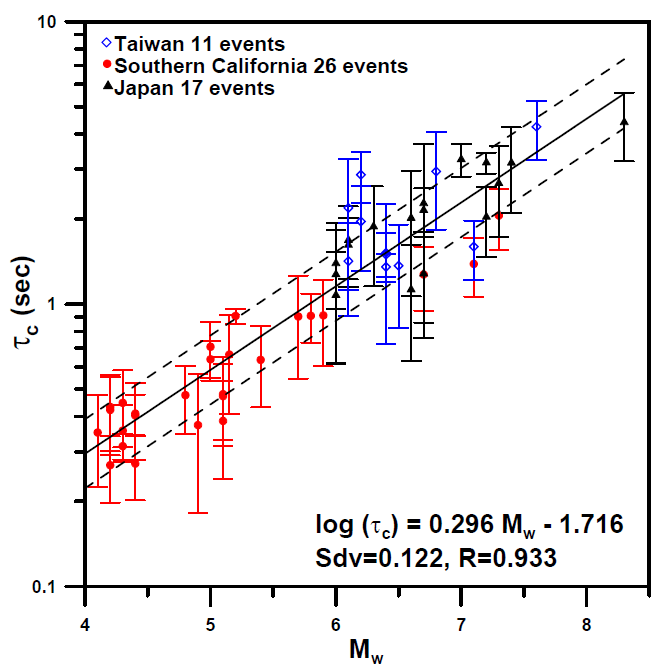
\includegraphics[width=0.7\linewidth]{img/kanamori2008_taoc.jpg} 
 \renewcommand{\figurename}{图} 
\caption{Kanamori et al. (2008)对于$\tau_{\mathrm{c}}$方法的研究(共使用54个地震事件)} 
%英文标题begin 
\addtocounter{figure}{-1} \vspace{-5pt} 
%\SetEnglishCaption 
\renewcommand{\figurename}{Fig} 
\caption{Kanamori et al. (2008) Study of the $\tau_{\mathrm{c}}$ method (using a total of 54 seismic events)} 
\renewcommand{\figurename}{图} 
%英文标题end 
\label{fig:network-device-influence.png} 
\end{figure}

\begin{equation}
\mathrm{r}=\frac{4 \pi^{2} \int_{0}^{\infty} f^{2}|\widehat{u}(f)|^{2} d f}{\int_{0}^{\infty}|a(f)|^{2} d f}=4 \pi^{2}\left\langle f^{2}\right\rangle
\end{equation}
\begin{equation}
\tau_{c}=\frac{1}{\sqrt{\left\langle f^{2}\right\rangle}}=\frac{2 \pi}{\sqrt{r}}
\end{equation}
其中$\widehat{u}(f)$为位移记录u(t)的频谱,$\left\langle f^{2}\right\rangle$为以$|\hat{u}(f)|^{2}$加权的频率平方平均值。在此定义下,$\tau_{\mathrm{c}}$即为P波初至时段内地震波的主要周期,也即是对P拐角频率的另一种特征估计,故可以用于估计断层破裂情况。与$\tau_{p}^{\max}$相比,$\tau_{\mathrm{c}}$方法更为稳定,需要更少的台站就可以得到稳定预测结果。在实践中,$\tau_{\mathrm{c}}$对于不同地区的差异性也更小 (Wu et al., 2005, 2008),在中国台湾、美国加州、日本地区都能得到一致结果。\\

\section{特征幅值类方法}

 \indent 使用地震台站记录的特征幅值预估震级的方式表面上与传统的震后震级确定的方法很接近,但从工作原理上来看两者有重要区别。由于时效性需求,特征幅值类方法要求使用短时间少量信息提取出特征幅值以预估震级,而震后确定工作更多完成的是标定工作。地震波在地球介质传播过程中,震动幅值会随着震中距的增大而衰减,特征幅值类的预估过程中就是利用了这种衰减关系。相同情况下由位移信息提取的幅值参数所得到的预估震级结果优于由速度、加速度信息所得的 (马强等, 2008),而台站记录中垂直向分量中的P波最为发育,故此类方法基本选择从台站垂直向记录中提取位移特征幅值。
 
 \indent 特征幅值类算法中,$\mathrm{P}_{\mathrm{d}}$方法最优。$\mathrm{P}_{\mathrm{d}}$一般定义为,台站垂直分量的位移记录在P波触发后3s时窗采用2阶高通巴特沃斯滤波器(常见低频截止频率为0.075Hz)滤波后的位移最大值(Wu et al., 2007)。$\mathrm{P}_{\mathrm{d}}$参数不仅与震级有关,也与地震动速度峰值PGV和加速度峰值PGA之间有相关性。$\mathrm{P}_{\mathrm{d}}$参数比较稳定,对地区差异性不敏感,经过震中距R修正后的规律在不同国家和地区都得到了统一验证,因此$\mathrm{P}_{\mathrm{d}}$参数可以作为预警目标区地震烈度估计的有利判据。$\mathrm{P}_{\mathrm{d}}$与$\mathrm{M}_{\mathrm{w}}$、PGV的关系可以表示为\\
\begin{equation}
\log \left(\mathrm{P}_{\mathrm{d}}\right)=\mathrm{A}_{1}+\mathrm{A}_{2} \mathrm{M}_{\mathrm{W}}+\mathrm{A}_{3} \log (\mathrm{R})
\end{equation}
\begin{equation}
\log \left(\mathrm{P}_{\mathrm{d}}\right)=\mathrm{B}_{1}+\mathrm{B}_{2} \log (\mathrm{PGV})
\end{equation}
 其中MW为矩震级,$\mathrm{A}_{\mathrm{i}}$和$\mathrm{B}_{\mathrm{i}}$分别为在局部地区$\mathrm{P}_{\mathrm{d}}$与$\mathrm{M}_{\mathrm{w}}$和$\mathrm{P}_{\mathrm{d}}$线性关系系数。$\mathrm{P}_{\mathrm{d}}$方法的劣势在于存在震级饱和现象。若设置时间窗长度为3s时,$\mathrm{P}_{\mathrm{d}}$方法的饱和震级约为6.5级,而当时间窗长度达到4s时饱和震级可以提高至7.0级 (Zollo et al., 2006)。\\
 

 
 